% ------------------------------------------------------------------------------
% 8. CRONOGRAMA
% ------------------------------------------------------------------------------
\subsection{8. Cronograma}\label{sec:cronograma}

\subsubsection{8.1. Plan de ejecución}\label{sec:plan_ejecucion}
% [INSTRUCCIÓN]: Fechas estimadas y duración para cada fase del proyecto.

\begin{figure}[htbp]
\caption{Diagrama de Gantt del plan de ejecución del proyecto: proceso unificado aplicado al Sistema de Gestión Integral del Comedor Universitario (24 de agosto al 30 de noviembre de 2026)}
\label{fig:cronograma}
\centering
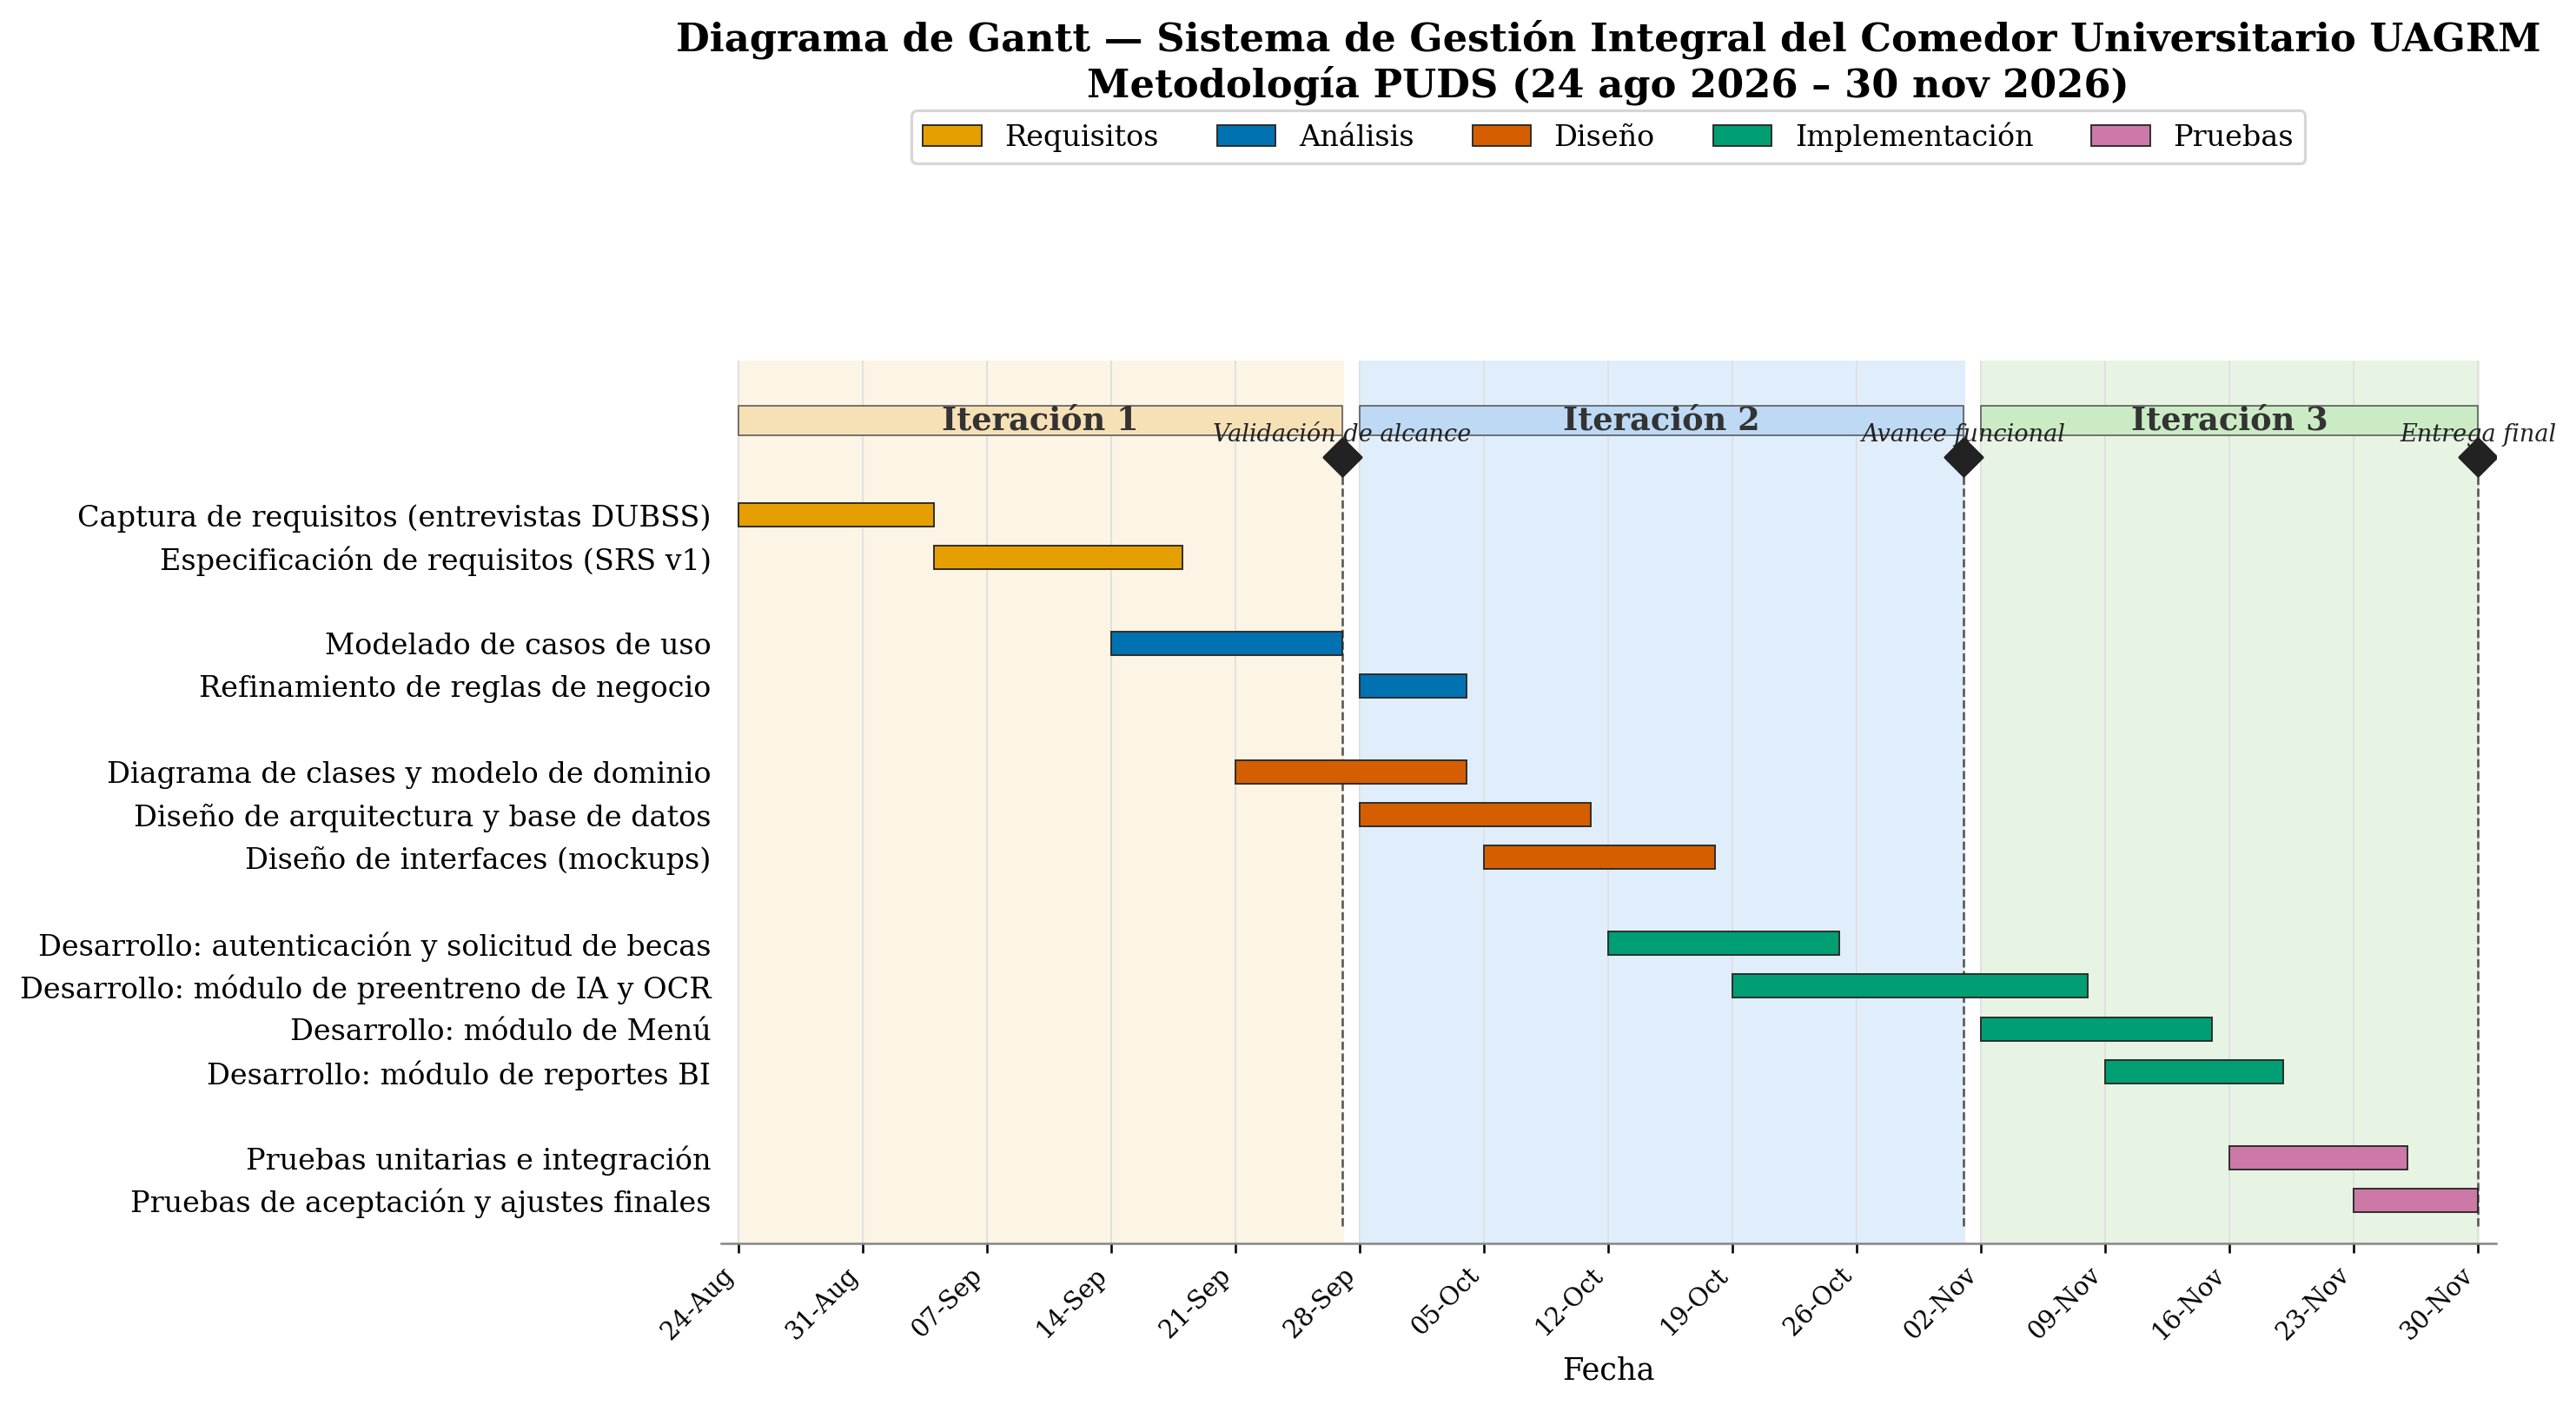
\includegraphics[width=\textwidth]{images/03_Cronograma_Gantt.png}
\smallskip
\noindent\raggedright\textit{Nota.} Elaboración propia. El diagrama detalla las fases del proyecto, sus duraciones estimadas en días hábiles y los hitos de validación de alcance, avance funcional y entrega final.
\end{figure}

\clearpage
\subsubsection{8.2. Hitos importantes}\label{sec:hitos_importantes}
% [INSTRUCCIÓN]: Hitos organizados según las tres fases de la materia.

Los hitos del proyecto se organizan según las tres fases de la materia (Fase 1, Fase 2 y Fase final), cada una con su avance o explicación y su presentación, como se detalla en la Tabla~\ref{tab:hitos}.

\begin{table}[H]
\caption{Hitos del proyecto según las fases de la materia}
\label{tab:hitos}
\begin{threeparttable}
\begin{tabular}{>{\raggedright\arraybackslash}p{2cm} >{\raggedright\arraybackslash}p{5cm} >{\raggedright\arraybackslash}p{5.5cm}}
\toprule
Fase & Actividad & Información adicional \\
\midrule
Fase 1 & Avance/explicación de los Capítulos 1 a 4, formato y bibliografía. & Tema del proyecto definido en la clase previa. \\
 & Presentación 1. & Revisión 1 del documento, hasta el Capítulo 4, en formato digital. \\
\midrule
Fase 2 & Avance/explicación de los Capítulos 5, 6 y 7. & Captura de requisitos, análisis y diseño. \\
 & Presentación 2. & Revisión 2 del documento, hasta el Capítulo 7, en formato digital. \\
\midrule
Fase final & Avance/explicación del Capítulo 8 en adelante. & Implementación y pruebas del sistema. \\
 & Presentación final del documento y del software, y defensa final. & Revisión final: documento completo y software desarrollado, en formato digital y físico, con presentación y defensa. \\
\bottomrule
\end{tabular}
\begin{tablenotes}
\item \textit{Nota.} Elaboración propia con base en las fases de avance definidas por la asignatura.
\end{tablenotes}
\end{threeparttable}
\end{table}
